\documentclass[a4paper,12pt]{article}
\usepackage{graphicx}
\title{How to Tie an Overhand Knot}
\author{}
\begin{document}
\maketitle 
\begin{abstract}
The overhand knot is one of the most fundamental knots and 
forms the basis of many others including the simple noose, overhand loop, 
angler's loop, reef knot, fisherman's knot and water knot. The overhand knot is 
very secure, to the point of jamming badly. It should be used if the knot is 
intended to be permanent. It is often used to prevent the end of a rope from 
unraveling. 
\end{abstract}

\section{Tying}

\begin{figure}[ht]
 \centering
 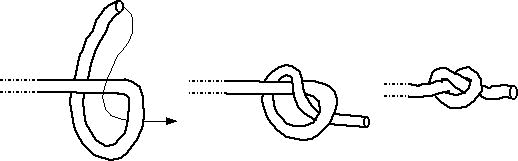
\includegraphics[scale=0.5]{tying.png}
 \caption{Tying the Overhand knot}\label{fig:overhand}
\end{figure}
There are a number of ways to tie the Overhand Knot, but the essential 
technique is shown in Fig. \ref{fig:overhand}.
\begin{itemize}
 \item Thumb method \--- create a loop and push the working end through the 
loop with your thumb.
 \item Overhand method \--- create a bight, by twisting the hand over at the 
wrist and sticking your hand in the hole, pinch the working end with your 
fingers and pull through the loop.
\end{itemize}

\section{Heraldry}

\begin{figure}[ht]
 \centering
 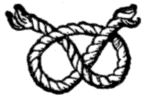
\includegraphics[scale=1]{heraldry.png}
 \caption{Stafford Knot}\label{fig:heraldry}
\end{figure}
In heraldry, the overhand knot is known as a ``Stafford knot'', 
due to use first as a heraldic badge by the 
``Lords of Stafford'', then as a general 
symbol of Staffordshire.\cite{heraldry} 
It is shown in Fig. \ref{fig:heraldry}.

The content for this document has been taken from the wiki \cite{wiki}.

\begin{thebibliography}{99}
\bibitem{wiki} http://en.wikipedia.org/wiki/Overhand\_knot as seen on April 7th 
2014
\bibitem{heraldry} Arthur Charles Fox-Davies, \emph{A Complete Guide to 
Heraldry} (1909), pp. 462, 469.
\end{thebibliography}



\end{document}
